\documentclass{beamer}

\mode<presentation> {
	\usetheme{Rochester}
	\setbeamertemplate{footline}[page number]
}

\usepackage{graphicx}
\usepackage{booktabs}

\title[Mind Map PIM]{Mind Map PIM}

\author{A-Cube-N}
\institute[UP]{
	Department of Computer Science, University of Pretoria
}
\date{\today}
\graphicspath{{pictures/}}

\begin{document}

\begin{frame}
	\titlepage
\end{frame}

\begin{frame}
	\frametitle{Overview}
	\tableofcontents
\end{frame}

\section{Concept}
	\subsection{Overview}
		\begin{frame}
		\frametitle{Project Overview}
			Mind Mapped PIM is a system that will process existing PIM platforms such as Facebook and Gmail and construct a mind map using that data. 
			The mind map will allow functionality of the sources e.g. send an email. It will be programmed in a way to display information that is most relevant to you at a particular time in your life.
		\end{frame}
	
	\subsection{What it is not}
		\begin{frame}
		\frametitle{What it is not}
			The Mind Map PIM is not a new social media platform. Rather it acts as a filter for your current social media platforms.  It will use intelligent algorithms to determine what information you would most likely want to see.
		\end{frame}
			
	\subsection{Platforms we will use}
		\begin{frame}
		\frametitle{Platforms we will use}
			We will make use of the following social media platforms by using the APIs that are provided by them:
			\begin{enumerate}
				\item Google services (priority)
					\begin{enumerate}
						\item Gmail
						\item Calendar
						\item Notes
						\item Plus
					\end{enumerate}
				\item Facebook
				\item LinkedIn
			\end{enumerate}
			We will be using dependency injection to implement the different platforms. This will enable future expansion to more platforms.
		\end{frame}
		
\section{Software Architecture}
	\subsection{Overview}
		\begin{frame}
		\frametitle{Software Architecture Overview}
			We will be using a layered system architecture to implement the system. This will allow us to better achieve:
			\begin{itemize}
				\item modularity
				\item flexibility
				\item scalability
				\item access limitation
			\end{itemize}
		\end{frame}
		
	\subsection{Requirements}
		\begin{frame}
		\frametitle{Some Software Architecture Requirements}
			\textbf{Usability} Very simple to use since users with varying computer literacy will use the system.\\
			\textbf{Performance} The system should be able to display information in real-time. New information should be displayed almost immediately.\\
			\textbf{Security} Since we are dealing with sensitive information it is vital that the best encryption and secure connections are used when communicating with external systems.\\
			\textbf{Reliability} The system will run seven days a week, twenty-four hours per day.
		\end{frame}
		
	\subsection{Design}
		\begin{frame}
		\frametitle{Software Architecture Design}
		 Model-View-Controller (MVC): this gives us many benefits mainly:
         	\textbf{Separation of design concerns:} Because of the decoupling of presentation, control, and data persistence and behavior, the application becomes more flexible; modifications to one component have minimal impact on other components.\\
        	\textbf{More easily maintainable and extensible:} Good structure can reduce code complexity. As such, code duplication is minimized.
        	\textbf{Promotes division of labour:} Developers with different skill sets are able to focus on their core skills and collaborate through clearly defined interfaces.\\
		\end{frame}
		
	\subsection{Technologies}
			\begin{frame}
			\frametitle{Technologies}
				Technologies we will be using:
				\begin{itemize}
					\item JavaEE
					\item TomEE (JavaEE version of Apache Tomcat)
					\item Google Parsey McParseFace (Natural Language Processor for English)
				\end{itemize}
			\end{frame}
			
		
	\subsection{Persistence}
		\begin{frame}
		\frametitle{Software Architecture Persistence}
			For persistence we will be using MongoDB. This choice was made on the fact that it will integrate better with our OO system and also the fact that services like Mind Map PIM has the potential to attract many users.
			Benefits include:
			\begin{itemize}
				\item high write loads
				\item good for Big Data scenarios
				\item highly scalable
				\item document orientated storage
			\end{itemize}
		\end{frame}
		
	\subsection{Interface}
		\begin{frame}
		\frametitle{Software Architecture Interface}
			The system will be accessed via a web interface (our primary goal) and an Android app (as a secondary goal). The mind map will be presented in a fashion similar to the way that musicroamer.com displays related music artists (see next slide).
			
			\begin{itemize}
				\item At the center is the root node.
				\item Each social media platform has a node going out from the root node.
				\item Relevant information is displayed about each platform.
				\item User can expand any node to find relevant information about that node.
				\item The user can specify a ply depth to specify how many 'branches' the mind map should allow from a main node
				\item Should a node allow functionality e.g. Facebook node allows you to comment, this functionality will be provided in a panel to the right of the mind map
			\end{itemize}
		\end{frame}
		\begin{frame}
		\frametitle{Software Architecture Interface}
			\begin{figure}
				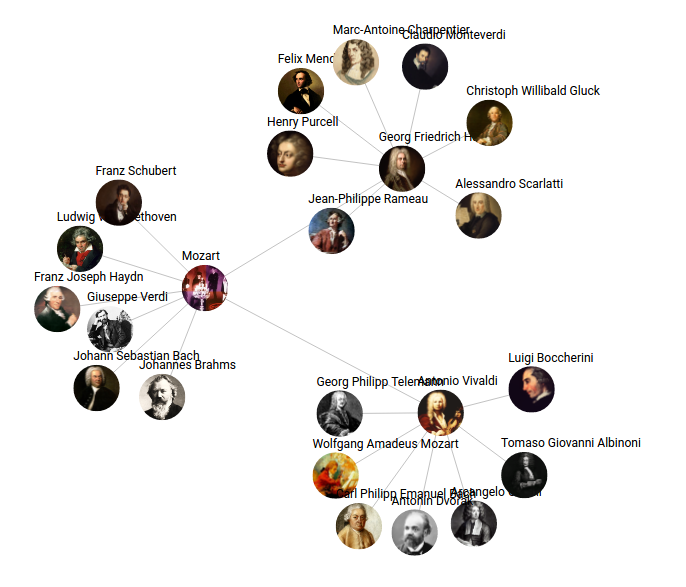
\includegraphics[scale=0.3]{musicroamer.png}
				\caption{Music Roamer layout of a music mind map}
			\end{figure}
		\end{frame}
		
		\begin{frame}
		\frametitle{Initial Design 1}
			\begin{figure}
				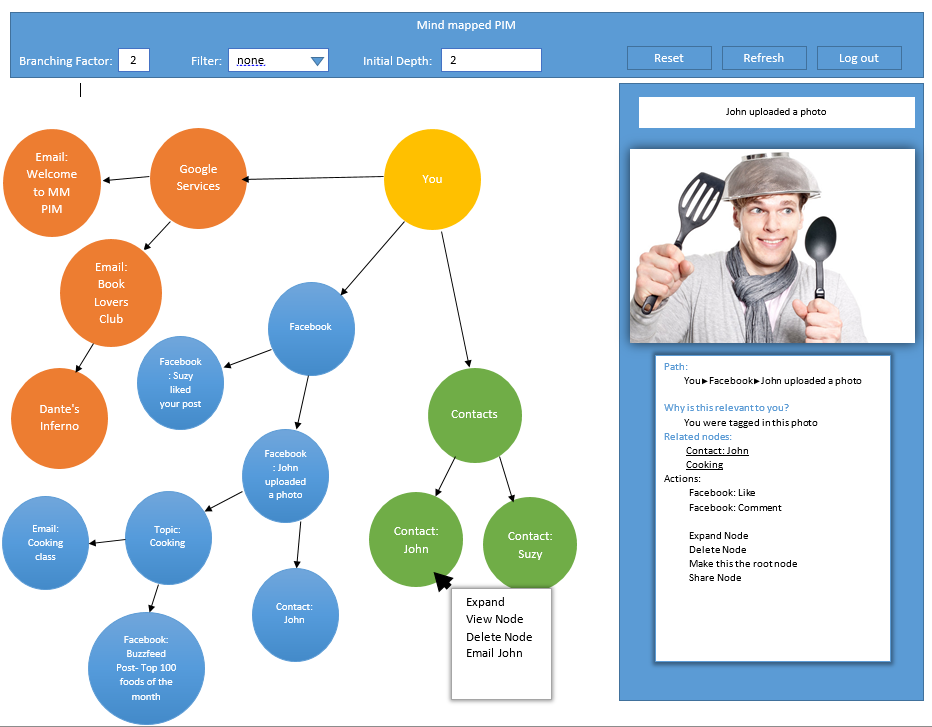
\includegraphics[scale=0.35]{initdesign.png}
			\end{figure}
		\end{frame}
		
		\begin{frame}
		\frametitle{Initial Design2}
			\begin{figure}
				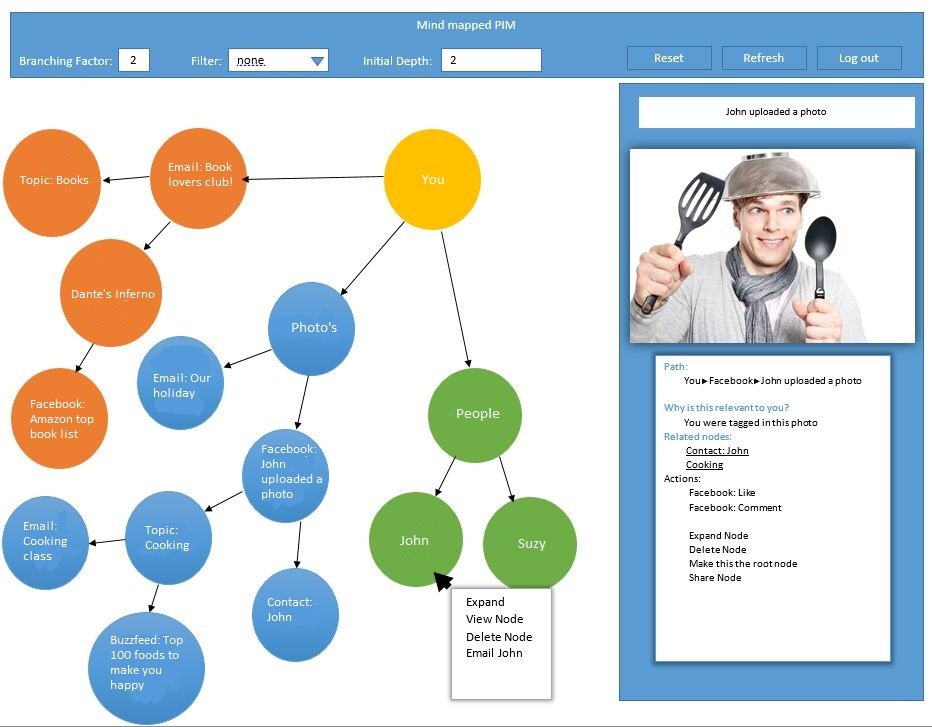
\includegraphics[scale=0.35]{initDesign2.jpg}
			\end{figure}
		\end{frame}
		\begin{frame}
			\Huge{\centerline{The End}}
		\end{frame}

\end{document} 
